\usepackage[a4paper,top=25mm,bottom=24mm,left=27mm,right=23mm,headheight=15pt]{geometry}
\usepackage{fontspec}
\setmainfont{Times New Roman}
\setsansfont{Times New Roman}
\setmonofont{Times New Roman}
\usepackage{amsmath,amssymb,graphicx,booktabs,array,longtable,float,tabularx}
\usepackage{unicode-math}
\setmathfont{Cambria Math}
\usepackage{indentfirst}
\usepackage[table]{xcolor}
\usepackage{enumitem,fancyhdr,titlesec,caption,subcaption,tcolorbox}
\usepackage{tikz}
\usetikzlibrary{arrows.meta,positioning,calc,fit,backgrounds}
\usepackage[numbers,sort&compress]{natbib}
\usepackage{placeins}\usepackage{hyperref}
\hypersetup{plainpages=false,colorlinks=true,linkcolor=black,citecolor=black,urlcolor=black,
 pdftitle={CO5087: Vietnamese news classification},pdfauthor={Dang Nguyen Tan Tai}}
\setlength{\parindent}{1cm}
\setlength{\parskip}{4pt}
\linespread{1.1}
\emergencystretch=4em
\raggedbottom
\pagestyle{fancy}
\fancyhf{}
\fancyhead[L]{\small CO5087: Phân loại tin tức}
\fancyhead[R]{\small Xử lý ngôn ngữ tự nhiên}
\fancyfoot[C]{\thepage}
\renewcommand{\headrulewidth}{0.4pt}
\fancypagestyle{plain}{\fancyhf{}\fancyfoot[C]{\thepage}\renewcommand{\headrulewidth}{0pt}}
\titleformat{\chapter}[hang]{\normalfont\LARGE\bfseries}{\thechapter.}{0.6em}{}
\titlespacing{\chapter}{0pt}{-8pt}{18pt}
\captionsetup{font=small,labelfont=bf}
\renewcommand{\contentsname}{Mục lục}
\renewcommand{\listfigurename}{Danh sách hình vẽ}
\renewcommand{\listtablename}{Danh sách bảng}
\renewcommand{\figurename}{Hình}
\renewcommand{\tablename}{Bảng}
\renewcommand{\bibname}{Tài liệu tham khảo}
\renewcommand{\appendixname}{Phụ lục}
\setlist[itemize]{topsep=3pt,itemsep=2pt,leftmargin=1.6em}
\tikzset{box/.style={draw=black,align=center,
 minimum height=12mm,text width=29mm,font=\small,fill=white},
 fc/.style={box},output/.style={box},
 flow/.style={-{Latex[length=2mm]},thick},
 note/.style={align=center,font=\footnotesize,text width=35mm}}
\newcommand{\ReportFigure}[3][.90]{\begin{figure}[tbp]\centering
\includegraphics[width=#1\linewidth,keepaspectratio]{#2}\caption{#3}\end{figure}}
\newcommand{\DataTable}[2]{\begin{table}[htbp]\centering\caption{#2}
\small\setlength{\tabcolsep}{4pt}\input{#1}\end{table}}
\newcommand{\Evidence}[1]{\begin{tcolorbox}[colback=white,colframe=black,
 boxrule=.5pt,arc=1mm]#1\end{tcolorbox}}
\setcounter{topnumber}{3}
\setcounter{bottomnumber}{2}
\setcounter{totalnumber}{4}
\renewcommand{\topfraction}{.88}
\renewcommand{\bottomfraction}{.8}
\renewcommand{\textfraction}{.1}
\renewcommand{\floatpagefraction}{.7}
% Publication-grade Monochrome TikZ Architectures for NLP Report
% Design Standards:
% 1. Pure monochrome (black, white, gray!5..15), Times New Roman / Cambria Math typography.
% 2. Maximum of 1 or 2 node sizes per diagram for clean academic rhythm.
% 3. Fixed, mathematically calculated inter-node distances (zero collision, zero overlapping).
% 4. Strict Manhattan orthogonal routing (-- , |- , -|), zero diagonal or slanted lines.
% 5. Text-minimized boxes with clean mathematical notation; detailed notes in bottom badges.

\tikzset{
  % Unified Academic Styles
  arch_box/.style={
    draw=black, line width=0.6pt, fill=white, rounded corners=2pt,
    align=center, inner sep=4pt, font=\small
  },
  arch_box_gray/.style={
    arch_box, fill=black!5
  },
  arch_box_dark/.style={
    arch_box, fill=black!12
  },
  arch_box_dashed/.style={
    arch_box, dashed, fill=black!2
  },
  arch_op/.style={
    draw=black, line width=0.6pt, circle, fill=white,
    inner sep=1.5pt, font=\footnotesize
  },
  arch_flow/.style={
    -{Latex[length=2.2mm,width=1.5mm]}, line width=0.7pt, draw=black
  },
  arch_line/.style={
    line width=0.7pt, draw=black
  },
  arch_badge/.style={
    draw=black!45, line width=0.5pt, rounded corners=2pt, fill=black!2,
    align=left, inner sep=4.5pt, font=\footnotesize
  }
}

% -----------------------------------------------------------------------------
% 1. PipelineDiagram: End-to-end NLP Overview
% Node Sizes: Exactly 1 size (30mm x 14mm) for all 8 pipeline steps.
% Fixed Spacing: dx = 38mm (gap = 8mm), dy = 22mm (gap = 8mm).
% -----------------------------------------------------------------------------
\newcommand{\PipelineDiagram}{
\begin{figure}[tbp]\centering
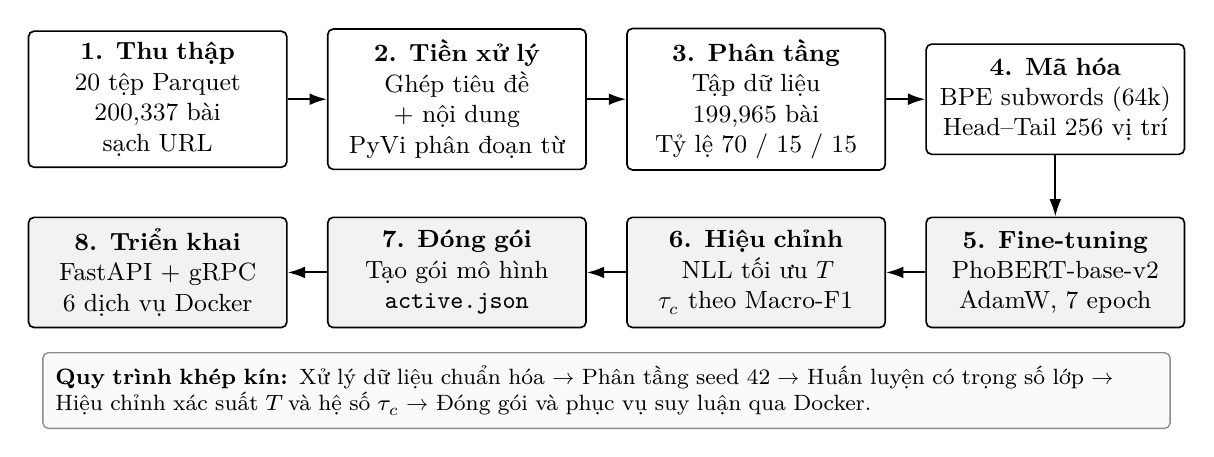
\begin{tikzpicture}
  % Row 1: Data Preparation & Preprocessing (Left to Right, y = 1.1)
  \node[arch_box, text width=30mm, minimum height=14mm] (p1) at (-5.7,1.1) {
    \textbf{1. Thu thập}\\
    20 tệp Parquet\\
    200,337 bài sạch URL
  };
  \node[arch_box, text width=30mm, minimum height=14mm] (p2) at (-1.9,1.1) {
    \textbf{2. Tiền xử lý}\\
    Ghép tiêu đề + nội dung\\
    PyVi phân đoạn từ
  };
  \node[arch_box, text width=30mm, minimum height=14mm] (p3) at (1.9,1.1) {
    \textbf{3. Phân tầng}\\
    Tập dữ liệu 199,965 bài\\
    Tỷ lệ 70 / 15 / 15
  };
  \node[arch_box, text width=30mm, minimum height=14mm] (p4) at (5.7,1.1) {
    \textbf{4. Mã hóa}\\
    BPE subwords (64k)\\
    Head--Tail 256 vị trí
  };

  % Row 2: Modeling, Calibration & Serving (Right to Left, y = -1.1)
  \node[arch_box_gray, text width=30mm, minimum height=14mm] (p5) at (5.7,-1.1) {
    \textbf{5. Fine-tuning}\\
    PhoBERT-base-v2\\
    AdamW, 7 epoch
  };
  \node[arch_box_gray, text width=30mm, minimum height=14mm] (p6) at (1.9,-1.1) {
    \textbf{6. Hiệu chỉnh}\\
    NLL tối ưu $T$\\
    $\tau_c$ theo Macro-F1
  };
  \node[arch_box_gray, text width=30mm, minimum height=14mm] (p7) at (-1.9,-1.1) {
    \textbf{7. Đóng gói}\\
    Tạo gói mô hình\\
    \texttt{active.json}
  };
  \node[arch_box_gray, text width=30mm, minimum height=14mm] (p8) at (-5.7,-1.1) {
    \textbf{8. Triển khai}\\
    FastAPI + gRPC\\
    6 dịch vụ Docker
  };

  % Strictly Orthogonal Connections (All horizontal gaps = 8mm, vertical drop = 8mm)
  \draw[arch_flow] (p1) -- (p2);
  \draw[arch_flow] (p2) -- (p3);
  \draw[arch_flow] (p3) -- (p4);
  \draw[arch_flow] (p4.south) -- (p5.north);
  \draw[arch_flow] (p5) -- (p6);
  \draw[arch_flow] (p6) -- (p7);
  \draw[arch_flow] (p7) -- (p8);

  % Bottom Invariant Badge
  \node[arch_badge, text width=140mm] (badge) at (0,-2.6) {
    \textbf{Quy trình khép kín:} Xử lý dữ liệu chuẩn hóa $\to$ Phân tầng seed 42 $\to$ Huấn luyện có trọng số lớp $\to$ Hiệu chỉnh xác suất $T$ và hệ số $\tau_c$ $\to$ Đóng gói và phục vụ suy luận qua Docker.
  };
\end{tikzpicture}
\caption{Quy trình NLP tổng thể từ dữ liệu thô đến hệ thống ứng dụng hỗ trợ biên tập.}
\end{figure}
}

% -----------------------------------------------------------------------------
% 2. SplitDiagram: Strict 3-Way Data Partitioning
% Node Sizes: Exactly 2 sizes:
%   - Size 1: Wide Banner (130mm x 11mm) for Master Corpus.
%   - Size 2: Partition & Role Boxes (38mm x 18mm) for all 6 columns.
% Fixed Spacing: dx = 48mm (gap = 10mm), dy = 26mm (gap = 8mm).
% -----------------------------------------------------------------------------
\newcommand{\SplitDiagram}{
\begin{figure}[tbp]\centering
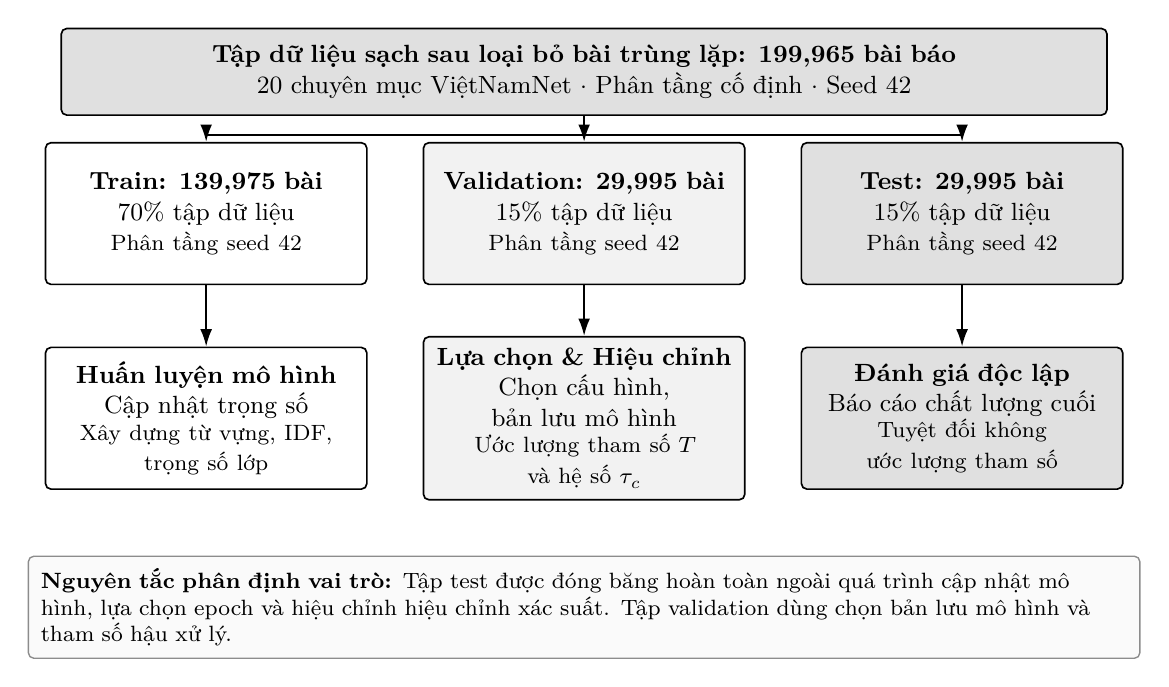
\begin{tikzpicture}
  % Stage 1: Filtered Master Corpus (y = 2.8)
  \node[arch_box_dark, text width=130mm, minimum height=11mm] (all) at (0,2.8) {
    \textbf{Tập dữ liệu sạch sau loại bỏ bài trùng lặp: 199,965 bài báo}\\
    20 chuyên mục ViệtNamNet $\cdot$ Phân tầng cố định $\cdot$ Seed 42
  };

  % Strictly Orthogonal Bus Coordinate (y = 2.0)
  \coordinate (splitbus) at (0,2.0);

  % Stage 2: Three Partitions (Symmetric, y = 1.0, height = 18mm)
  \node[arch_box, text width=38mm, minimum height=18mm] (train) at (-4.8,1.0) {
    \textbf{Train: 139,975 bài}\\
    \small 70\% tập dữ liệu\\
    \footnotesize Phân tầng seed 42
  };
  \node[arch_box_gray, text width=38mm, minimum height=18mm] (val) at (0,1.0) {
    \textbf{Validation: 29,995 bài}\\
    \small 15\% tập dữ liệu\\
    \footnotesize Phân tầng seed 42
  };
  \node[arch_box_dark, text width=38mm, minimum height=18mm] (test) at (4.8,1.0) {
    \textbf{Test: 29,995 bài}\\
    \small 15\% tập dữ liệu\\
    \footnotesize Phân tầng seed 42
  };

  % Stage 3: Operational Roles (y = -1.6, height = 18mm, exact 8mm gap from Row 2!)
  \node[arch_box, text width=38mm, minimum height=18mm] (fit) at (-4.8,-1.6) {
    \textbf{Huấn luyện mô hình}\\
    \small Cập nhật trọng số\\
    \footnotesize Xây dựng từ vựng, IDF,\\trọng số lớp
  };
  \node[arch_box_gray, text width=38mm, minimum height=18mm] (select) at (0,-1.6) {
    \textbf{Lựa chọn \& Hiệu chỉnh}\\
    \small Chọn cấu hình, bản lưu mô hình\\
    \footnotesize Ước lượng tham số $T$\\và hệ số $\tau_c$
  };
  \node[arch_box_dark, text width=38mm, minimum height=18mm] (score) at (4.8,-1.6) {
    \textbf{Đánh giá độc lập}\\
    \small Báo cáo chất lượng cuối\\
    \footnotesize Tuyệt đối không\\ước lượng tham số
  };

  % Strictly Orthogonal Bus Connections (Start on splitbus y=2.0)
  \draw[arch_line] (all.south) -- (splitbus);
  \draw[arch_line] (-4.8,2.0) -- (4.8,2.0);
  \draw[arch_flow] (-4.8,2.0) -- (train.north);
  \draw[arch_flow] (splitbus) -- (val.north);
  \draw[arch_flow] (4.8,2.0) -- (test.north);

  % Vertical Connections to Roles (Exact 8mm straight arrows)
  \draw[arch_flow] (train) -- (fit);
  \draw[arch_flow] (val) -- (select);
  \draw[arch_flow] (test) -- (score);

  % Bottom Invariant Badge (y = -4.0, generous 8mm clearance from role boxes)
  \node[arch_badge, text width=138mm] (badge) at (0,-4.0) {
    \textbf{Nguyên tắc phân định vai trò:} Tập test được đóng băng hoàn toàn ngoài quá trình cập nhật mô hình, lựa chọn epoch và hiệu chỉnh hiệu chỉnh xác suất. Tập validation dùng chọn bản lưu mô hình và tham số hậu xử lý.
  };
\end{tikzpicture}
\caption{Ba tập dữ liệu có vai trò tách biệt; tập test nằm ngoài cập nhật, chọn bản lưu mô hình và hiệu chỉnh.}
\end{figure}
}

% -----------------------------------------------------------------------------
% 3. PreprocessDiagram: Text Normalization Pipeline
% Node Sizes: Exactly 1 size (128mm x 11mm) for all 4 stages.
% Fixed Spacing: node distance = 7mm.
% -----------------------------------------------------------------------------
\newcommand{\PreprocessDiagram}{
\begin{figure}[tbp]\centering
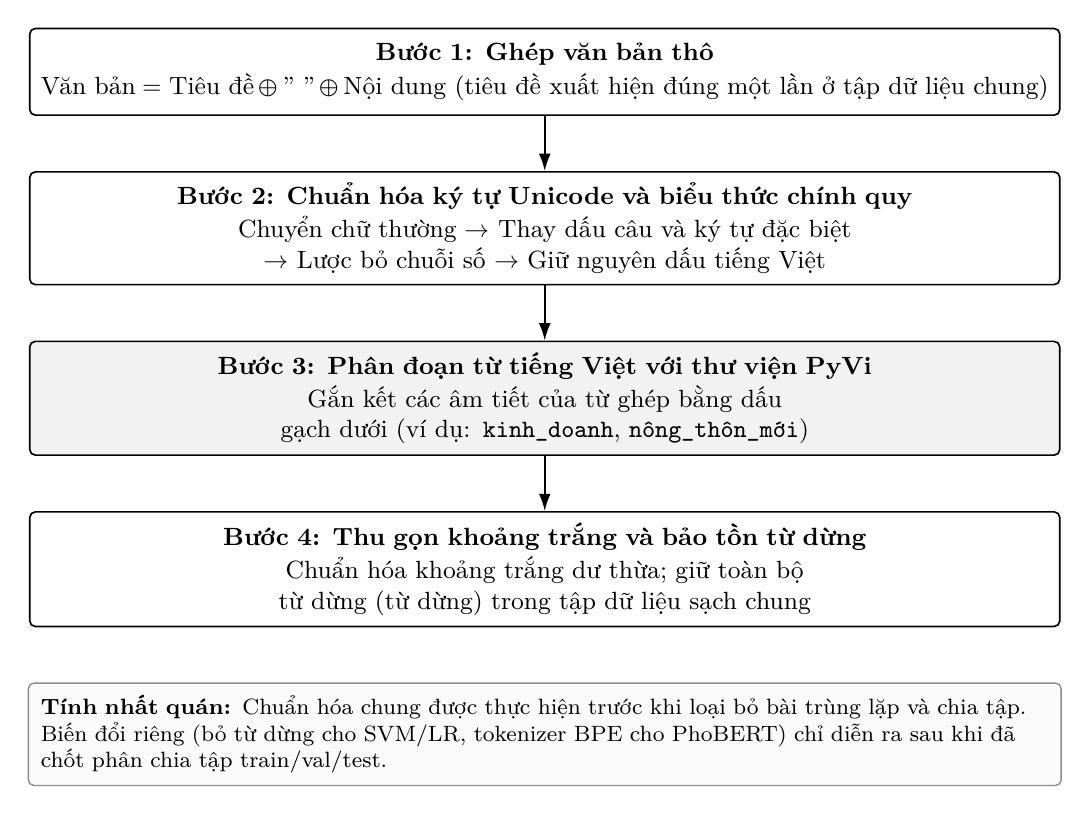
\begin{tikzpicture}[node distance=7mm]
  % Stage 1: Input text assembly
  \node[arch_box, text width=128mm, minimum height=11mm] (s1) {
    \textbf{Bước 1: Ghép văn bản thô}\\[1pt]
    $\text{Văn bản} = \text{Tiêu đề} \oplus \text{" "} \oplus \text{Nội dung}$ (tiêu đề xuất hiện đúng một lần ở tập dữ liệu chung)
  };

  % Stage 2: Normalization
  \node[arch_box, text width=128mm, minimum height=11mm, below=of s1] (s2) {
    \textbf{Bước 2: Chuẩn hóa ký tự Unicode và biểu thức chính quy}\\[1pt]
    Chuyển chữ thường $\to$ Thay dấu câu và ký tự đặc biệt $\to$ Lược bỏ chuỗi số $\to$ Giữ nguyên dấu tiếng Việt
  };

  % Stage 3: Word Segmentation
  \node[arch_box_gray, text width=128mm, minimum height=11mm, below=of s2] (s3) {
    \textbf{Bước 3: Phân đoạn từ tiếng Việt với thư viện PyVi}\\[1pt]
    Gắn kết các âm tiết của từ ghép bằng dấu gạch dưới (ví dụ: \texttt{kinh\_doanh}, \texttt{nông\_thôn\_mới})
  };

  % Stage 4: Whitespace and Corpus Delivery
  \node[arch_box, text width=128mm, minimum height=11mm, below=of s3] (s4) {
    \textbf{Bước 4: Thu gọn khoảng trắng và bảo tồn từ dừng}\\[1pt]
    Chuẩn hóa khoảng trắng dư thừa; giữ toàn bộ từ dừng (từ dừng) trong tập dữ liệu sạch chung
  };

  % Strictly Orthogonal Straight Arrows (Fixed 7mm length)
  \draw[arch_flow] (s1) -- (s2);
  \draw[arch_flow] (s2) -- (s3);
  \draw[arch_flow] (s3) -- (s4);

  % Bottom Badge
  \node[arch_badge, text width=128mm, below=7mm of s4] (b) {
    \textbf{Tính nhất quán:} Chuẩn hóa chung được thực hiện trước khi loại bỏ bài trùng lặp và chia tập. Biến đổi riêng (bỏ từ dừng cho SVM/LR, tokenizer BPE cho PhoBERT) chỉ diễn ra sau khi đã chốt phân chia tập train/val/test.
  };
\end{tikzpicture}
\caption{Chuẩn hóa chung trước loại bỏ bài trùng lặp; biến đổi riêng của từng mô hình diễn ra sau khi chốt tập dữ liệu.}\label{fig:preprocess}
\end{figure}
}

% -----------------------------------------------------------------------------
% 4. CorpusAuditDiagram: Data Cleaning Tree
% Node Sizes: Exactly 2 sizes:
%   - Size 1: Wide Banner (128mm x 12mm) for Stages 1, 2, 4, 5, 6.
%   - Size 2: Column Box (38mm x 15mm) for Stage 3 (3 branches).
% Fixed Spacing: Symmetric center at x = 0, fixed vertical steps.
% -----------------------------------------------------------------------------
\newcommand{\CorpusAuditDiagram}{
\begin{figure}[tbp]\centering
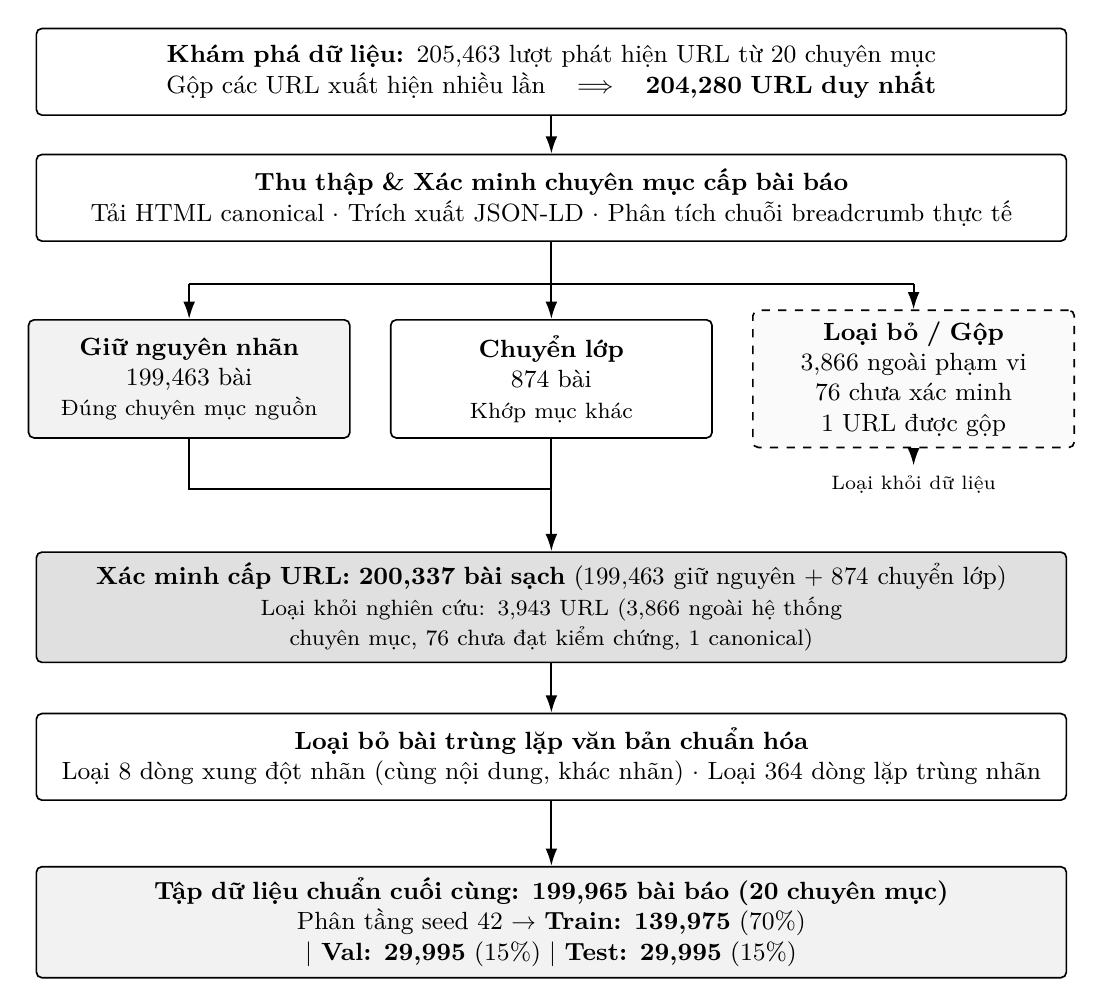
\begin{tikzpicture}
  % Stage 1: Raw Discovery (y = 5.5)
  \node[arch_box, text width=128mm, minimum height=11mm] (raw) at (0,5.5) {
    \textbf{Khám phá dữ liệu:} 205,463 lượt phát hiện URL từ 20 chuyên mục\\
    Gộp các URL xuất hiện nhiều lần $\implies$ \textbf{204,280 URL duy nhất}
  };

  % Stage 2: HTML Extraction & Verification (y = 3.9, 5mm gap from raw)
  \node[arch_box, text width=128mm, minimum height=11mm] (verify) at (0,3.9) {
    \textbf{Thu thập \& Xác minh chuyên mục cấp bài báo}\\
    Tải HTML canonical $\cdot$ Trích xuất \mbox{JSON-LD} $\cdot$ Phân tích chuỗi breadcrumb thực tế
  };

  % Stage 3: Three Branches (y = 1.6, height = 15mm)
  \node[arch_box_gray, text width=38mm, minimum height=15mm] (same) at (-4.6,1.6) {
    \textbf{Giữ nguyên nhãn}\\
    199,463 bài\\
    \footnotesize Đúng chuyên mục nguồn
  };
  \node[arch_box, text width=38mm, minimum height=15mm] (move) at (0,1.6) {
    \textbf{Chuyển lớp}\\
    874 bài\\
    \footnotesize Khớp mục khác
  };
  \node[arch_box_dashed, text width=38mm, minimum height=15mm] (drop) at (4.6,1.6) {
    \textbf{Loại bỏ / Gộp}\\
    3,866 ngoài phạm vi\\
    76 chưa xác minh\\
    1 URL được gộp
  };

  % Stage 4: Clean URL Aggregation (Wide Banner, y = -1.3, height = 12mm)
  \node[arch_box_dark, text width=128mm, minimum height=12mm] (clean) at (0,-1.3) {
    \textbf{Xác minh cấp URL: 200,337 bài sạch} ($199{,}463\text{ giữ nguyên} + 874\text{ chuyển lớp}$)\\
    \footnotesize Loại khỏi nghiên cứu: 3,943 URL (3,866 ngoài hệ thống chuyên mục, 76 chưa đạt kiểm chứng, 1 canonical)
  };

  % Stage 5: Text Deduplication (Wide Banner, y = -3.2, height = 11mm)
  \node[arch_box, text width=128mm, minimum height=11mm] (dedup) at (0,-3.2) {
    \textbf{Loại bỏ bài trùng lặp văn bản chuẩn hóa}\\
    Loại 8 dòng xung đột nhãn (cùng nội dung, khác nhãn) $\cdot$ Loại 364 dòng lặp trùng nhãn
  };

  % Stage 6: Final Corpus & Split (Wide Banner, y = -5.3, height = 12mm)
  \node[arch_box_gray, text width=128mm, minimum height=12mm] (corpus) at (0,-5.3) {
    \textbf{Tập dữ liệu chuẩn cuối cùng: 199,965 bài báo (20 chuyên mục)}\\
    Phân tầng seed 42 $\to$ \textbf{Train: 139,975} (70\%) $\mid$ \textbf{Val: 29,995} (15\%) $\mid$ \textbf{Test: 29,995} (15\%)
  };

  % Routing: Strictly Orthogonal
  \draw[arch_flow] (raw) -- (verify);

  % Branching from verify (bus at y = 2.8)
  \coordinate (vbus) at (0, 2.8);
  \draw[arch_line] (verify.south) -- (vbus);
  \draw[arch_line] (-4.6, 2.8) -- (4.6, 2.8);
  \draw[arch_flow] (-4.6, 2.8) -- (same.north);
  \draw[arch_flow] (vbus) -- (move.north);
  \draw[arch_flow] (4.6, 2.8) -- (drop.north);

  % Merging branches: 'same' and 'move' merge into clean (bus at y = 0.2)
  \coordinate (cbus) at (0, 0.2);
  \draw[arch_line] (same.south) -- (-4.6, 0.2) -- (cbus);
  \draw[arch_line] (move.south) -- (cbus);
  \draw[arch_flow] (cbus) -- (clean.north);

  % Excluded branch: drop terminates outside with generous clearance from clean
  \draw[arch_flow, dashed] (drop.south) -- (4.6, 0.5) node[below, font=\scriptsize] {Loại khỏi dữ liệu};

  % Sequential Spine: Clean to Dedup to Corpus (Strictly vertical straight drops)
  \draw[arch_flow] (clean) -- (dedup);
  \draw[arch_flow] (dedup) -- (corpus);

\end{tikzpicture}
\caption{Xác minh chuyên mục và tạo tập dữ liệu; nhánh loại/gộp không đi vào dữ liệu huấn luyện.}\label{fig:corpus-audit}
\end{figure}
}

% -----------------------------------------------------------------------------
% 5. MethodFamiliesDiagram: 3 Representation Families & 4 Models
% Node Sizes: Exactly 2 sizes:
%   - Size 1: Wide Banner (136mm x 10mm) for Input and Output.
%   - Size 2: Grid Column Box (42mm x 16mm) for all 9 intermediate nodes.
% Fixed Spacing: dx = 47mm (gap = 5mm), dy = 22mm (gap = 6mm).
% -----------------------------------------------------------------------------
\newcommand{\MethodFamiliesDiagram}{
\begin{figure}[tbp]\centering
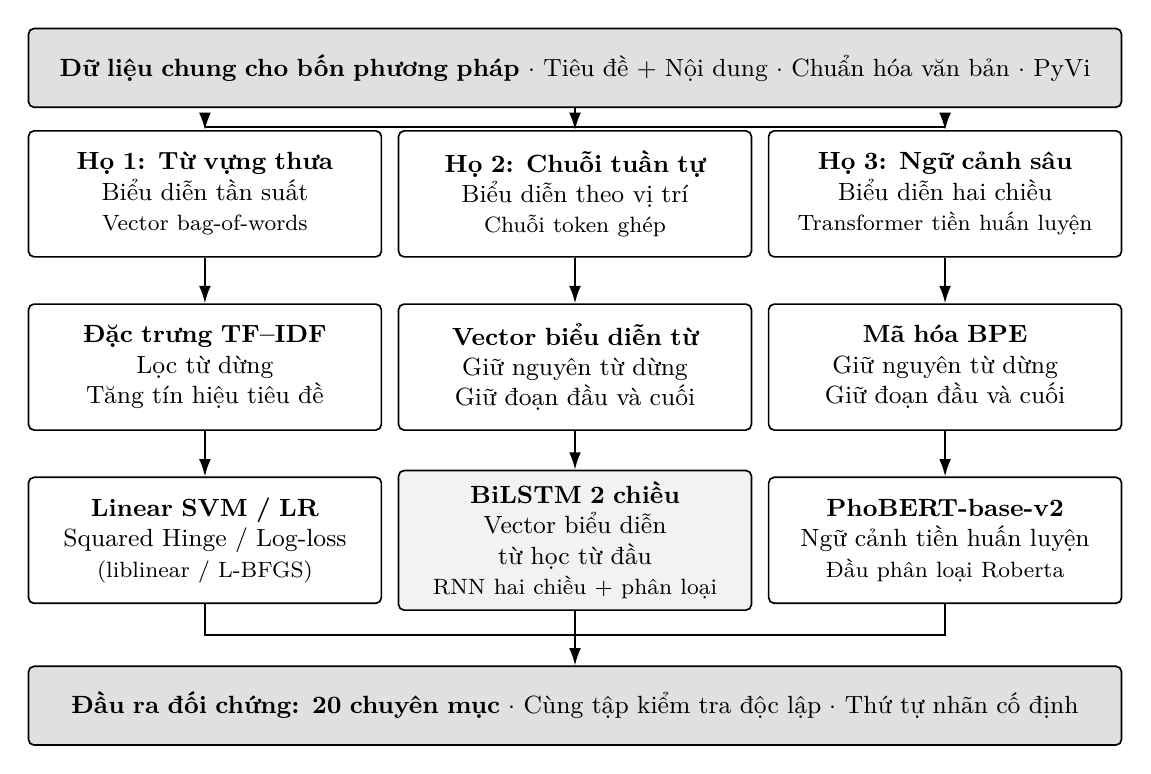
\begin{tikzpicture}
  % Common Input Node (y = 0)
  \node[arch_box_dark, text width=136mm, minimum height=10mm] (input) at (0,0) {
    \textbf{Dữ liệu chung cho bốn phương pháp} $\cdot$ Tiêu đề + Nội dung $\cdot$ Chuẩn hóa văn bản $\cdot$ PyVi
  };

  % Level 1: Representation Families (y = -1.6, height = 16mm)
  \node[arch_box, text width=42mm, minimum height=16mm] (fam1) at (-4.7,-1.6) {
    \textbf{Họ 1: Từ vựng thưa}\\
    \small Biểu diễn tần suất\\
    \footnotesize Vector bag-of-words
  };
  \node[arch_box, text width=42mm, minimum height=16mm] (fam2) at (0,-1.6) {
    \textbf{Họ 2: Chuỗi tuần tự}\\
    \small Biểu diễn theo vị trí\\
    \footnotesize Chuỗi token ghép
  };
  \node[arch_box, text width=42mm, minimum height=16mm] (fam3) at (4.7,-1.6) {
    \textbf{Họ 3: Ngữ cảnh sâu}\\
    \small Biểu diễn hai chiều\\
    \footnotesize Transformer tiền huấn luyện
  };

  % Level 2: Features & Vocabularies (y = -3.8, height = 16mm, exact 6mm gap!)
  \node[arch_box, text width=42mm, minimum height=16mm] (rep1) at (-4.7,-3.8) {
    \textbf{Đặc trưng TF--IDF}\\
    Lọc từ dừng\\
    Tăng tín hiệu tiêu đề
  };
  \node[arch_box, text width=42mm, minimum height=16mm] (rep2) at (0,-3.8) {
    \textbf{Vector biểu diễn từ}\\
    Giữ nguyên từ dừng\\
    Giữ đoạn đầu và cuối
  };
  \node[arch_box, text width=42mm, minimum height=16mm] (rep3) at (4.7,-3.8) {
    \textbf{Mã hóa BPE}\\
    Giữ nguyên từ dừng\\
    Giữ đoạn đầu và cuối
  };

  % Level 3: Model Architectures (y = -6.0, height = 16mm, exact 6mm gap!)
  \node[arch_box, text width=42mm, minimum height=16mm] (mod1) at (-4.7,-6.0) {
    \textbf{Linear SVM / LR}\\
    \small Squared Hinge / Log-loss\\
    \footnotesize (liblinear / L-BFGS)
  };
  \node[arch_box_gray, text width=42mm, minimum height=16mm] (mod2) at (0,-6.0) {
    \textbf{BiLSTM 2 chiều}\\
    \small Vector biểu diễn từ học từ đầu\\
    \footnotesize RNN hai chiều + phân loại
  };
  \node[arch_box, text width=42mm, minimum height=16mm] (mod3) at (4.7,-6.0) {
    \textbf{PhoBERT-base-v2}\\
    \small Ngữ cảnh tiền huấn luyện\\
    \footnotesize Đầu phân loại Roberta
  };

  % Common Output Node (y = -8.1, height = 10mm)
  \node[arch_box_dark, text width=136mm, minimum height=10mm] (out) at (0,-8.1) {
    \textbf{Đầu ra đối chứng: 20 chuyên mục} $\cdot$ Cùng tập kiểm tra độc lập $\cdot$ Thứ tự nhãn cố định
  };

  % Top Bus at y = -0.75
  \coordinate (inbus) at (0,-0.75);
  \draw[arch_line] (input.south) -- (inbus);
  \draw[arch_line] (-4.7,-0.75) -- (4.7,-0.75);
  \draw[arch_flow] (-4.7,-0.75) -- (fam1.north);
  \draw[arch_flow] (inbus) -- (fam2.north);
  \draw[arch_flow] (4.7,-0.75) -- (fam3.north);

  % Vertical Sequential Flows (All exact 6mm vertical arrows)
  \draw[arch_flow] (fam1) -- (rep1);
  \draw[arch_flow] (rep1) -- (mod1);

  \draw[arch_flow] (fam2) -- (rep2);
  \draw[arch_flow] (rep2) -- (mod2);

  \draw[arch_flow] (fam3) -- (rep3);
  \draw[arch_flow] (rep3) -- (mod3);

  % Bottom Bus at y = -7.2 (Strictly Orthogonal)
  \coordinate (outbus) at (0,-7.2);
  \draw[arch_line] (mod1.south) |- (outbus);
  \draw[arch_line] (mod2.south) -- (outbus);
  \draw[arch_line] (mod3.south) |- (outbus);
  \draw[arch_flow] (outbus) -- (out.north);

\end{tikzpicture}
\caption{Ba họ biểu diễn và bốn quy trình phân loại. Phần văn bản quan sát, tiền huấn luyện và ngân sách tối ưu khác nhau.}\label{fig:method_families}
\end{figure}
}

% -----------------------------------------------------------------------------
% 6. BiLSTMDiagram: BiLSTM Baseline Architecture (Figure fig:bilstm_arch)
% Node Sizes: Exactly 1 rectangular size (21mm x 14mm) for all 6 stages.
% Fixed Spacing: Clean 6mm horizontal gaps between all nodes.
% -----------------------------------------------------------------------------
\newcommand{\BiLSTMDiagram}{
\begin{figure}[tbp]\centering
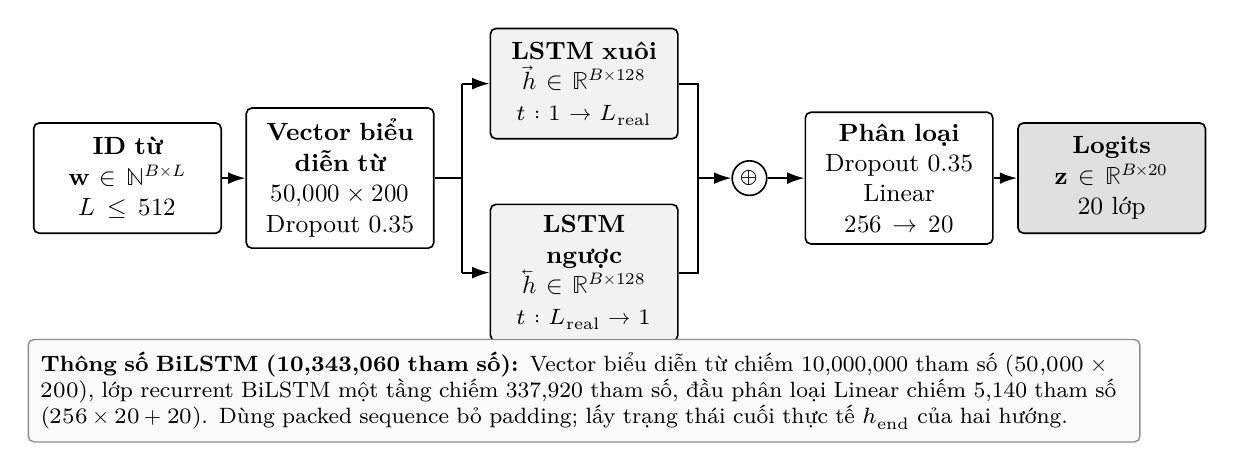
\begin{tikzpicture}
  % Input Tokens (center -5.8, width 21mm -> [-6.85, -4.75])
  \node[arch_box, text width=21mm, minimum height=14mm] (tok) at (-5.8,0) {
    \textbf{ID từ}\\
    $\mathbf{w} \in \mathbb{N}^{B \times L}$\\
    $L \le 512$
  };

  % Word Embedding (center -3.1, width 21mm -> [-4.15, -2.05])
  \node[arch_box, text width=21mm, minimum height=14mm] (emb) at (-3.1,0) {
    \textbf{Vector biểu diễn từ}\\
    $50{,}000 \times 200$\\
    Dropout 0.35
  };

  % BiLSTM Recurrent Layers (center 0.0, width 21mm -> [-1.05, +1.05])
  \node[arch_box_gray, text width=21mm, minimum height=14mm] (fw) at (0,1.2) {
    \textbf{LSTM xuôi}\\
    $\overrightarrow{h} \in \mathbb{R}^{B \times 128}$\\
    \footnotesize $t: 1 \to L_{\text{real}}$
  };
  \node[arch_box_gray, text width=21mm, minimum height=14mm] (bw) at (0,-1.2) {
    \textbf{LSTM ngược}\\
    $\overleftarrow{h} \in \mathbb{R}^{B \times 128}$\\
    \footnotesize $t: L_{\text{real}} \to 1$
  };

  % Concatenation Operator (diameter 6mm, center at x = 2.1)
  \node[arch_op] (cat) at (2.1,0) {$\oplus$};

  % Classification Head (center 4.0, width 21mm -> [2.95, 5.05])
  \node[arch_box, text width=21mm, minimum height=14mm] (head) at (4.0,0) {
    \textbf{Phân loại}\\
    Dropout 0.35\\
    Linear $256 \to 20$
  };

  % Logits Output (center 6.7, width 21mm -> [5.65, 7.75])
  \node[arch_box_dark, text width=21mm, minimum height=14mm] (out) at (6.7,0) {
    \textbf{Logits}\\
    $\mathbf{z} \in \mathbb{R}^{B \times 20}$\\
    20 lớp
  };

  % Strictly Orthogonal Routing: tok to emb (6mm clean arrow)
  \draw[arch_flow] (tok) -- (emb);

  % Emb to Forward and Backward: Split bus at x = -1.55 (5mm from emb.east, 5mm from fw.west!)
  \coordinate (emb_split) at (-1.55, 0);
  \draw[arch_line] (emb.east) -- (emb_split);
  \draw[arch_line] (emb_split) -- (-1.55, 1.2);
  \draw[arch_flow] (-1.55, 1.2) -- (fw.west);
  \draw[arch_line] (emb_split) -- (-1.55, -1.2);
  \draw[arch_flow] (-1.55, -1.2) -- (bw.west);

  % Forward and Backward to Concat: Join bus at x = 1.45 (4mm from fw.east, 4mm from cat.west!)
  \coordinate (cat_join) at (1.45, 0);
  \draw[arch_line] (fw.east) -- (1.45, 1.2) -- (cat_join);
  \draw[arch_line] (bw.east) -- (1.45, -1.2) -- (cat_join);
  \draw[arch_flow] (cat_join) -- (cat.west);

  % Concat to Head (6mm clean arrow)
  \draw[arch_flow] (cat) -- (head);

  % Head to Out (6mm clean arrow)
  \draw[arch_flow] (head) -- (out);

  % Bottom Parameter Badge (y = -2.7, generous clearance)
  \node[arch_badge, text width=138mm] (badge) at (0,-2.7) {
    \textbf{Thông số BiLSTM (10,343,060 tham số):} Vector biểu diễn từ chiếm 10,000,000 tham số ($50{,}000 \times 200$), lớp recurrent BiLSTM một tầng chiếm 337,920 tham số, đầu phân loại Linear chiếm 5,140 tham số ($256 \times 20 + 20$). Dùng packed sequence bỏ padding; lấy trạng thái cuối thực tế $h_{\text{end}}$ của hai hướng.
  };
\end{tikzpicture}
\caption{BiLSTM thực thi trong notebook: vector biểu diễn từ học từ đầu, packed sequence, ghép hidden cuối hai hướng và đầu phân loại 20 lớp. Dropout vector biểu diễn từ được lược trong khối để giữ sơ đồ gọn.}\label{fig:bilstm_arch}
\end{figure}
}

% -----------------------------------------------------------------------------
% 7. HeadTailDiagram: PhoBERT Head-Tail Truncation
% Node Sizes: Exactly 2 sizes:
%   - Size 1: Wide Banner (138mm x 9mm) for Raw BPE Sequence.
%   - Size 2: Uniform Segment Box (22mm x 14mm) for each segment.
% -----------------------------------------------------------------------------
\newcommand{\HeadTailDiagram}{
\begin{figure}[tbp]\centering
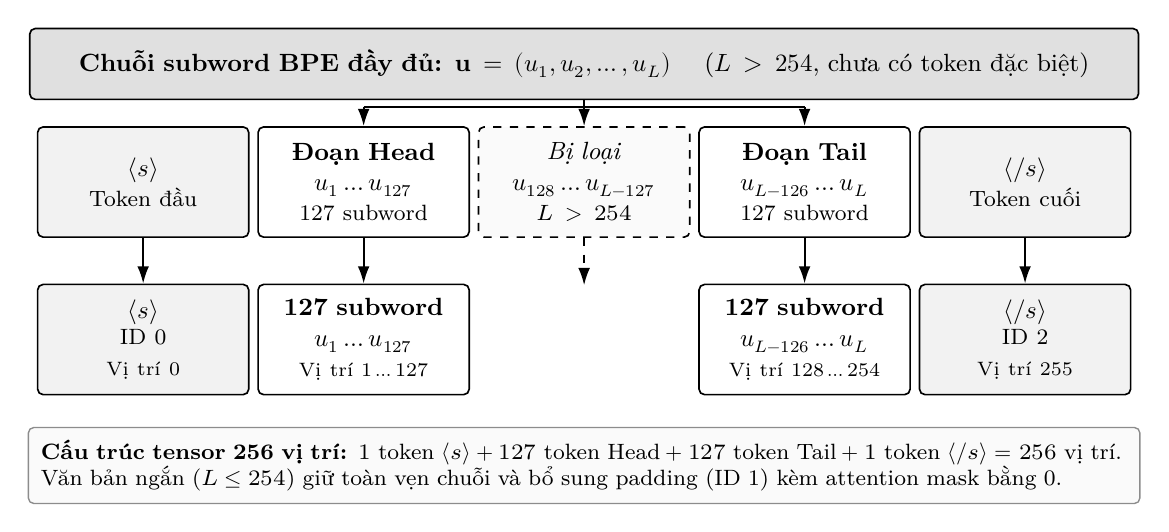
\begin{tikzpicture}
  % Top: Raw BPE Sequence Representation (Wide Banner, y = 2.5)
  \node[arch_box_dark, text width=138mm, minimum height=9mm] (raw) at (0,2.5) {
    \textbf{Chuỗi subword BPE đầy đủ:} $\mathbf{u} = (u_1, u_2, \ldots, u_L)$ \quad ($L > 254$, chưa có token đặc biệt)
  };

  % Visual Partitioning (y = 1.0, 5 identical 24mm boxes, uniform 4mm gap)
  \node[arch_box_gray, text width=24mm, minimum height=14mm] (p_cls) at (-5.6,1.0) {
    $\langle s\rangle$\\
    \footnotesize Token đầu
  };
  \node[arch_box, text width=24mm, minimum height=14mm] (p_head) at (-2.8,1.0) {
    \textbf{Đoạn Head}\\
    $u_1 \dots u_{127}$\\
    \footnotesize 127 subword
  };
  \node[arch_box_dashed, text width=24mm, minimum height=14mm] (p_mid) at (0,1.0) {
    \textit{Bị loại}\\
    \small $u_{128} \dots u_{L-127}$\\
    \footnotesize $L > 254$
  };
  \node[arch_box, text width=24mm, minimum height=14mm] (p_tail) at (2.8,1.0) {
    \textbf{Đoạn Tail}\\
    $u_{L-126} \dots u_L$\\
    \footnotesize 127 subword
  };
  \node[arch_box_gray, text width=24mm, minimum height=14mm] (p_sep) at (5.6,1.0) {
    $\langle/ s\rangle$\\
    \footnotesize Token cuối
  };

  % Bottom: Assembled 256-token Tensor (y = -1.0, 8mm gap from Row 1!)
  \node[arch_box_gray, text width=24mm, minimum height=14mm] (t_cls) at (-5.6,-1.0) {
    $\langle s\rangle$\\
    \footnotesize ID 0\\
    \scriptsize Vị trí 0
  };
  \node[arch_box, text width=24mm, minimum height=14mm] (t_head) at (-2.8,-1.0) {
    \textbf{127 subword}\\
    $u_1 \dots u_{127}$\\
    \scriptsize Vị trí $1 \dots 127$
  };
  \node[arch_box, text width=24mm, minimum height=14mm] (t_tail) at (2.8,-1.0) {
    \textbf{127 subword}\\
    $u_{L-126} \dots u_L$\\
    \scriptsize Vị trí $128 \dots 254$
  };
  \node[arch_box_gray, text width=24mm, minimum height=14mm] (t_sep) at (5.6,-1.0) {
    $\langle/ s\rangle$\\
    \footnotesize ID 2\\
    \scriptsize Vị trí 255
  };

  % Orthogonal Routing: Top to Partition
  \coordinate (rawbus) at (0, 1.95);
  \draw[arch_line] (raw.south) -- (rawbus);
  \draw[arch_line] (-2.8, 1.95) -- (2.8, 1.95);
  \draw[arch_flow] (-2.8, 1.95) -- (p_head.north);
  \draw[arch_flow] (2.8, 1.95) -- (p_tail.north);
  \draw[arch_flow] (rawbus) -- (p_mid.north);

  % Strictly Vertical Straight Drops to Assembled Tensor (8mm vertical arrows)
  \draw[arch_flow] (p_cls) -- (t_cls);
  \draw[arch_flow] (p_head) -- (t_head);
  \draw[arch_flow] (p_tail) -- (t_tail);
  \draw[arch_flow] (p_sep) -- (t_sep);

  % Middle omission drop (dashed)
  \draw[arch_flow, dashed] (p_mid.south) -- ++(0,-0.6);

  % Invariant Badge (y = -2.6)
  \node[arch_badge, text width=138mm] (b) at (0,-2.6) {
    \textbf{Cấu trúc tensor 256 vị trí:} $1 \text{ token } \langle s\rangle + 127 \text{ token Head} + 127 \text{ token Tail} + 1 \text{ token } \langle/ s\rangle = 256 \text{ vị trí}$. Văn bản ngắn ($L \le 254$) giữ toàn vẹn chuỗi và bổ sung padding (ID 1) kèm attention mask bằng 0.
  };
\end{tikzpicture}
\caption{Cách ghép Head--Tail; dấu token được minh họa theo ký hiệu của tokenizer PhoBERT.}
\end{figure}
}

% -----------------------------------------------------------------------------
% 8. EncoderDiagram: PhoBERT Architecture & Classification Head
% Node Sizes: Exactly 1 size (128mm x 11mm) for all 6 stages.
% Fixed Spacing: node distance = 6mm.
% -----------------------------------------------------------------------------
\newcommand{\EncoderDiagram}{
\begin{figure}[tbp]\centering
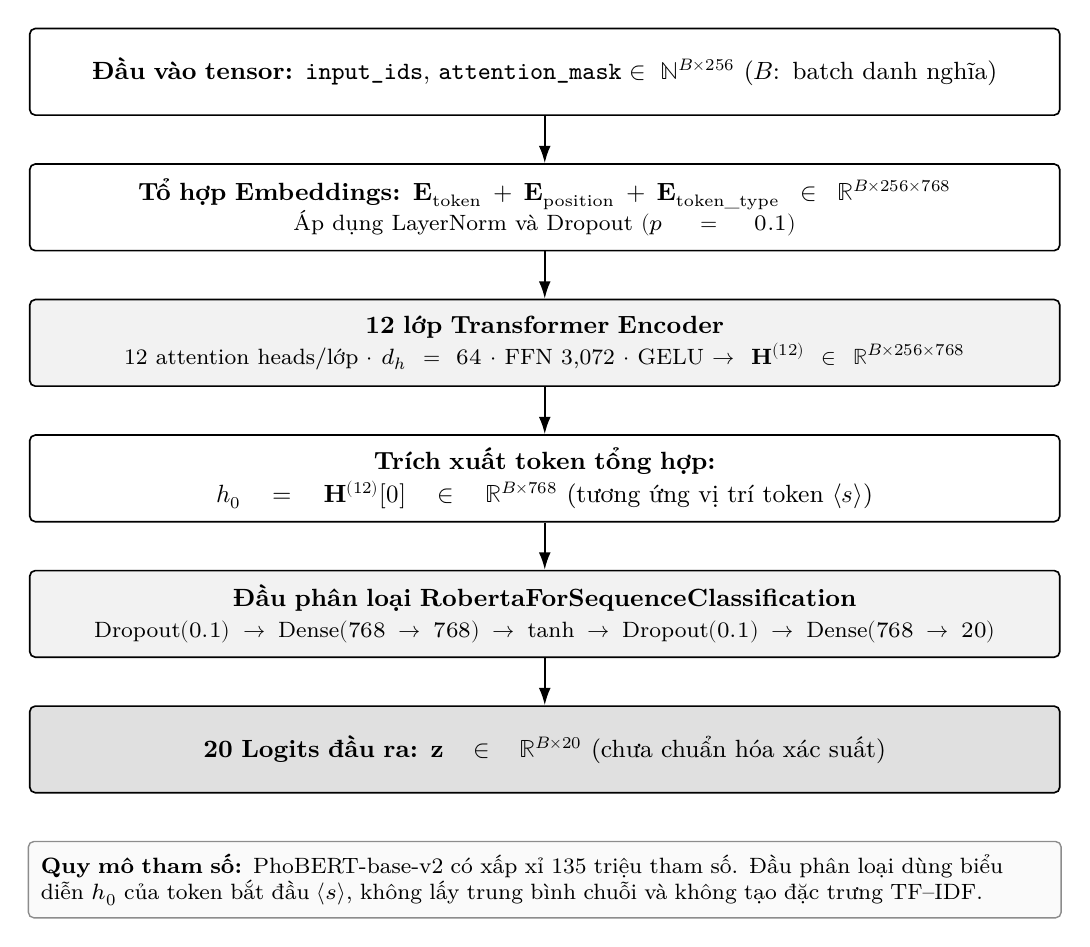
\begin{tikzpicture}[node distance=6mm]
  % Stage 1: Input Tensors
  \node[arch_box, text width=128mm, minimum height=11mm] (e1) {
    \textbf{Đầu vào tensor:} \texttt{input\_ids}, \texttt{attention\_mask} $\in \mathbb{N}^{B \times 256}$ ($B$: batch danh nghĩa)
  };

  % Stage 2: Embeddings
  \node[arch_box, text width=128mm, minimum height=11mm, below=of e1] (e2) {
    \textbf{Tổ hợp Embeddings:} $\mathbf{E}_{\text{token}} + \mathbf{E}_{\text{position}} + \mathbf{E}_{\text{token\_type}} \in \mathbb{R}^{B \times 256 \times 768}$\\
    \footnotesize Áp dụng LayerNorm và Dropout $(p=0.1)$
  };

  % Stage 3: Transformer Stack
  \node[arch_box_gray, text width=128mm, minimum height=11mm, below=of e2] (e3) {
    \textbf{12 lớp Transformer Encoder}\\
    \footnotesize 12 attention heads/lớp $\cdot$ $d_h=64$ $\cdot$ FFN 3,072 $\cdot$ GELU $\to \mathbf{H}^{(12)} \in \mathbb{R}^{B \times 256 \times 768}$
  };

  % Stage 4: First Token Extraction
  \node[arch_box, text width=128mm, minimum height=11mm, below=of e3] (e4) {
    \textbf{Trích xuất token tổng hợp:}\\[1pt]
    $h_0 = \mathbf{H}^{(12)}[0] \in \mathbb{R}^{B \times 768}$ (tương ứng vị trí token $\langle s\rangle$)
  };

  % Stage 5: Classification Head
  \node[arch_box_gray, text width=128mm, minimum height=11mm, below=of e4] (e5) {
    \textbf{Đầu phân loại RobertaForSequenceClassification}\\
    \footnotesize $\text{Dropout}(0.1) \to \text{Dense}(768 \to 768) \to \tanh \to \text{Dropout}(0.1) \to \text{Dense}(768 \to 20)$
  };

  % Stage 6: Output Logits
  \node[arch_box_dark, text width=128mm, minimum height=11mm, below=of e5] (e6) {
    \textbf{20 Logits đầu ra:} $\mathbf{z} \in \mathbb{R}^{B \times 20}$ (chưa chuẩn hóa xác suất)
  };

  % Strictly Orthogonal Straight Connections (All fixed 6mm vertical arrows)
  \draw[arch_flow] (e1) -- (e2);
  \draw[arch_flow] (e2) -- (e3);
  \draw[arch_flow] (e3) -- (e4);
  \draw[arch_flow] (e4) -- (e5);
  \draw[arch_flow] (e5) -- (e6);

  % Badge
  \node[arch_badge, text width=128mm, below=6mm of e6] (b) {
    \textbf{Quy mô tham số:} PhoBERT-base-v2 có xấp xỉ 135 triệu tham số. Đầu phân loại dùng biểu diễn $h_0$ của token bắt đầu $\langle s\rangle$, không lấy trung bình chuỗi và không tạo đặc trưng TF--IDF.
  };
\end{tikzpicture}
\caption{PhoBERT và đầu phân loại trong RobertaForSequenceClassification.}
\end{figure}
}

% -----------------------------------------------------------------------------
% 9. AttentionDiagram: Scaled Dot-Product & Multi-Head Attention
% Node Sizes: Exactly 2 sizes:
%   - Size 1: Wide Layer Box (112mm x 12mm) for H, Att, Res1, Res2, Out.
%   - Size 2: Projection Box (24mm x 12mm) for Q, K, V.
% Fixed Spacing: Symmetric center at x = 0, fixed vertical spacing.
% -----------------------------------------------------------------------------
\newcommand{\AttentionDiagram}{
\begin{figure}[tbp]\centering
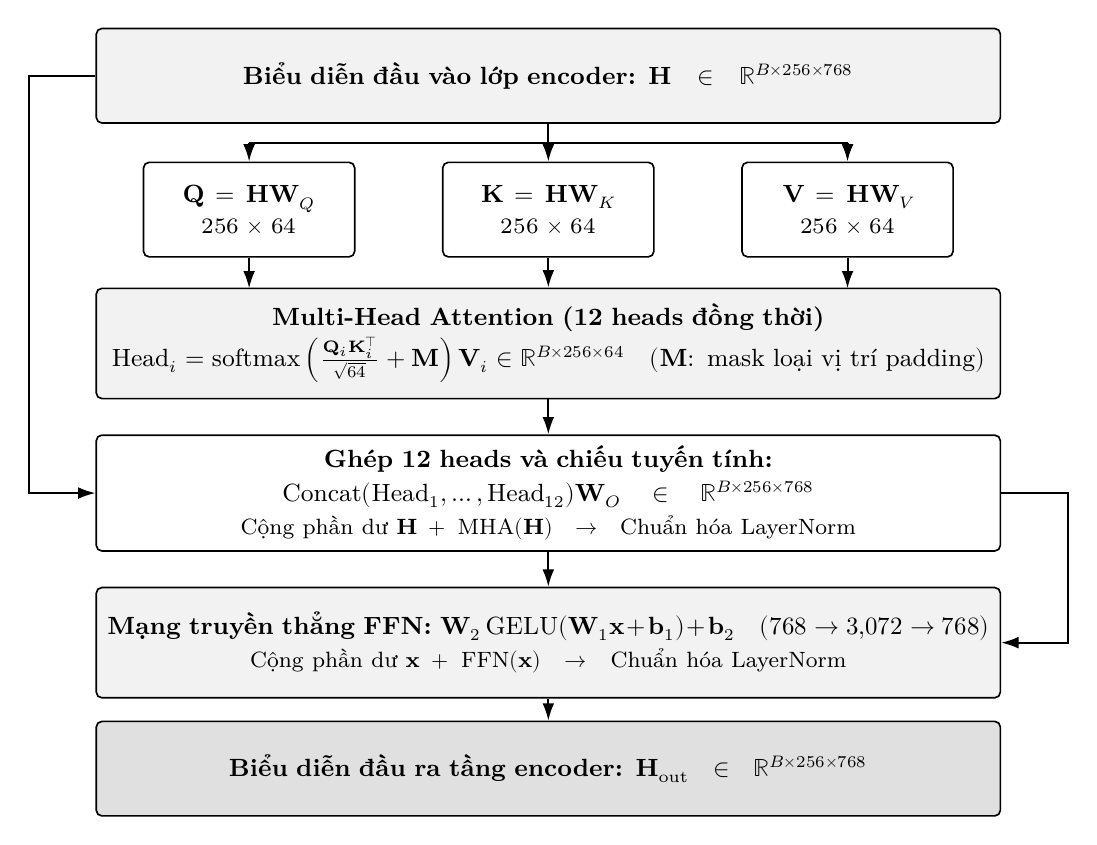
\begin{tikzpicture}
  % Stage 1: Input Hidden States (y = 4.4, width 112mm -> [-5.6, +5.6])
  \node[arch_box_gray, text width=112mm, minimum height=12mm] (h) at (0,4.4) {
    \textbf{Biểu diễn đầu vào lớp encoder:} $\mathbf{H} \in \mathbb{R}^{B \times 256 \times 768}$
  };

  % Stage 2: Linear Projections for Q, K, V (y = 2.7, width 24mm each)
  \node[arch_box, text width=24mm, minimum height=12mm] (q) at (-3.8,2.7) {
    $\mathbf{Q} = \mathbf{H}\mathbf{W}_Q$\\
    \footnotesize $256 \times 64$
  };
  \node[arch_box, text width=24mm, minimum height=12mm] (k) at (0,2.7) {
    $\mathbf{K} = \mathbf{H}\mathbf{W}_K$\\
    \footnotesize $256 \times 64$
  };
  \node[arch_box, text width=24mm, minimum height=12mm] (v) at (3.8,2.7) {
    $\mathbf{V} = \mathbf{H}\mathbf{W}_V$\\
    \footnotesize $256 \times 64$
  };

  % Stage 3: Multi-Head Scaled Dot-Product Attention (y = 1.0, width 112mm)
  \node[arch_box_gray, text width=112mm, minimum height=14mm] (att) at (0,1.0) {
    \textbf{Multi-Head Attention (12 heads đồng thời)}\\[1pt]
    $\text{Head}_i = \operatorname{softmax}\left(\frac{\mathbf{Q}_i \mathbf{K}_i^\top}{\sqrt{64}} + \mathbf{M}\right)\mathbf{V}_i \in \mathbb{R}^{B \times 256 \times 64} \quad (\mathbf{M}\text{: mask loại vị trí padding})$
  };

  % Stage 4: Projection, Residual Connection & LayerNorm (y = -0.9, width 112mm)
  \node[arch_box, text width=112mm, minimum height=14mm] (res1) at (0,-0.9) {
    \textbf{Ghép 12 heads và chiếu tuyến tính:}\\[1pt]
    $\operatorname{Concat}(\text{Head}_1, \ldots, \text{Head}_{12})\mathbf{W}_O \in \mathbb{R}^{B \times 256 \times 768}$\\[1pt]
    \footnotesize Cộng phần dư $\mathbf{H} + \text{MHA}(\mathbf{H}) \to \text{Chuẩn hóa LayerNorm}$
  };

  % Stage 5: Feed-Forward Network & LayerNorm (y = -2.8, width 112mm)
  \node[arch_box_gray, text width=112mm, minimum height=14mm] (res2) at (0,-2.8) {
    \textbf{Mạng truyền thẳng FFN:} $\mathbf{W}_2\operatorname{GELU}(\mathbf{W}_1 \mathbf{x} + \mathbf{b}_1) + \mathbf{b}_2 \quad (768 \to 3{,}072 \to 768)$\\[1pt]
    \footnotesize Cộng phần dư $\mathbf{x} + \text{FFN}(\mathbf{x}) \to \text{Chuẩn hóa LayerNorm}$
  };

  % Stage 6: Output Hidden States (y = -4.4, width 112mm)
  \node[arch_box_dark, text width=112mm, minimum height=12mm] (out) at (0,-4.4) {
    \textbf{Biểu diễn đầu ra tầng encoder:} $\mathbf{H}_{\text{out}} \in \mathbb{R}^{B \times 256 \times 768}$
  };

  % Bus from H to Q, K, V (Bus at y = 3.55)
  \coordinate (h_split) at (0,3.55);
  \draw[arch_line] (h.south) -- (h_split);
  \draw[arch_line] (-3.8,3.55) -- (3.8,3.55);
  \draw[arch_flow] (-3.8,3.55) -- (q.north);
  \draw[arch_flow] (h_split) -- (k.north);
  \draw[arch_flow] (3.8,3.55) -- (v.north);

  % From Q, K, V into att: Strictly parallel vertical drops
  \draw[arch_flow] (q.south) -- (-3.8, 1.7);
  \draw[arch_flow] (k.south) -- (att.north);
  \draw[arch_flow] (v.south) -- (3.8, 1.7);

  % Vertical Core Path
  \draw[arch_flow] (att) -- (res1);
  \draw[arch_flow] (res1) -- (res2);
  \draw[arch_flow] (res2) -- (out);

  % Residual 1 Bypass: clean outer Manhattan route (10mm clearance from widest box)
  \draw[arch_flow] (h.west) -- (-6.6, 4.4) |- (res1.west);

  % Residual 2 Bypass: clean outer Manhattan route (10mm clearance from widest box)
  \draw[arch_flow] (res1.east) -- (6.6, -0.9) |- (res2.east);

\end{tikzpicture}
\caption{Tính toán bên trong một lớp encoder; mask loại vị trí padding khỏi attention.}\label{fig:attention_layer}
\end{figure}
}

% -----------------------------------------------------------------------------
% 10. TrainDiagram: Iteration Loop & Gradient Accumulation
% Node Sizes: Exactly 2 sizes:
%   - Size 1: Mini-batch Steps 1..4 (28mm x 15mm)
%   - Size 2: Epoch Bản lưu mô hình Steps 5..6 (40mm x 15mm)
% Fixed Spacing: dx = 36mm (gap = 8mm), dy = 24mm (gap = 9mm).
% -----------------------------------------------------------------------------
\newcommand{\TrainDiagram}{
\begin{figure}[tbp]\centering
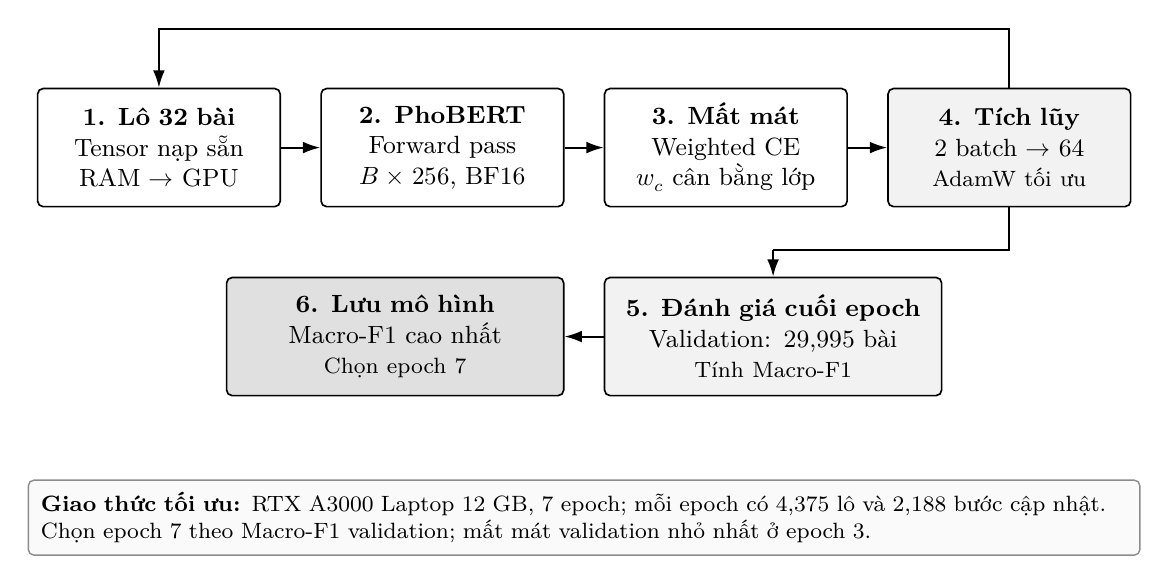
\begin{tikzpicture}
  % Row 1: Training Iteration (Left to Right, y = 1.2, width = 28mm)
  \node[arch_box, text width=28mm, minimum height=15mm] (b) at (-5.4,1.2) {
    \textbf{1. Lô 32 bài}\\
    Tensor nạp sẵn\\
    RAM $\to$ GPU
  };
  \node[arch_box, text width=28mm, minimum height=15mm] (m) at (-1.8,1.2) {
    \textbf{2. PhoBERT}\\
    Forward pass\\
    $B \times 256$, BF16
  };
  \node[arch_box, text width=28mm, minimum height=15mm] (l) at (1.8,1.2) {
    \textbf{3. Mất mát}\\
    Weighted CE\\
    $w_c$ cân bằng lớp
  };
  \node[arch_box_gray, text width=28mm, minimum height=15mm] (a) at (5.4,1.2) {
    \textbf{4. Tích lũy}\\
    \small 2 batch $\to$ 64\\
    \footnotesize AdamW tối ưu
  };

  % Row 2: Validation & Bản lưu mô hình (y = -1.2, width = 40mm, exact 9mm gap from Row 1!)
  \node[arch_box_dark, text width=40mm, minimum height=15mm] (c) at (-2.4,-1.2) {
    \textbf{6. Lưu mô hình}\\
    Macro-F1 cao nhất\\
    \footnotesize Chọn epoch 7
  };
  \node[arch_box_gray, text width=40mm, minimum height=15mm] (e) at (2.4,-1.2) {
    \textbf{5. Đánh giá cuối epoch}\\
    Validation: 29,995 bài\\
    \footnotesize Tính Macro-F1
  };

  % Forward Flow Row 1 (Clean 8mm horizontal arrows)
  \draw[arch_flow] (b) -- (m);
  \draw[arch_flow] (m) -- (l);
  \draw[arch_flow] (l) -- (a);

  % Batch Accumulation Loop: Up 8mm, left across to b.north.x, down into b.north
  \draw[arch_flow] (a.north) -- ++(0, 0.75) -| (b.north);

  % Epoch End Transition: Clean Manhattan drop at y = -0.1 (well clear of node a)
  \coordinate (epoch_turn) at (2.4, -0.1);
  \draw[arch_line] (a.south) |- (epoch_turn);
  \draw[arch_flow] (epoch_turn) -- (e.north);

  % Bản lưu mô hình selection: horizontal straight left (Clean 8mm arrow)
  \draw[arch_flow] (e) -- (c);

  % Bottom Invariant Badge (y = -3.5, generous 8mm clearance from Row 2)
  \node[arch_badge, text width=138mm] (badge) at (0,-3.5) {
    \textbf{Giao thức tối ưu:} RTX A3000 Laptop 12 GB, 7 epoch; mỗi epoch có 4,375 lô và 2,188 bước cập nhật. Chọn epoch 7 theo Macro-F1 validation; mất mát validation nhỏ nhất ở epoch 3.
  };
\end{tikzpicture}
\caption{Huấn luyện có tích lũy gradient và chọn bản lưu mô hình theo Macro-F1.}
\end{figure}
}

% -----------------------------------------------------------------------------
% 11. CalibrationDiagram: Temperature Scaling & Editorial Policy
% Node Sizes: Exactly 2 sizes:
%   - Size 1: Pipeline Stage Box (28mm x 14mm) for Row 1 (4 boxes).
%   - Size 2: Policy Routing Box (60mm x 14mm) for Row 2 (2 boxes).
% Fixed Spacing: dx = 36mm (gap = 8mm in Row 1), dy = 24mm (gap = 10mm between rows).
% -----------------------------------------------------------------------------
\newcommand{\CalibrationDiagram}{
\begin{figure}[htbp]\centering
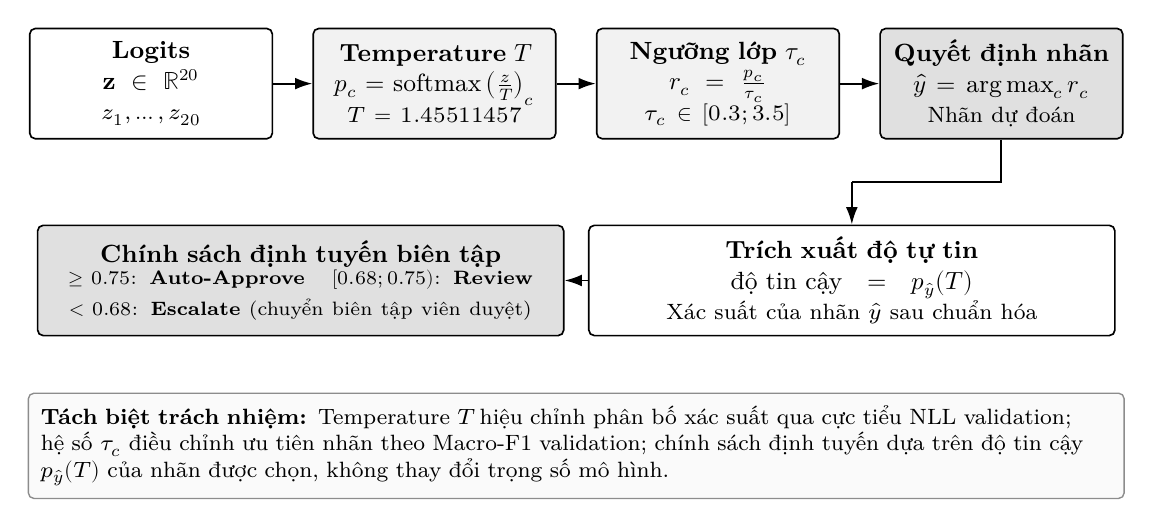
\begin{tikzpicture}
  % Stage 1: Pipeline Nodes (Horizontal, y = 1.3, width = 28mm)
  \node[arch_box, text width=28mm, minimum height=14mm] (z) at (-5.4,1.3) {
    \textbf{Logits}\\
    $\mathbf{z} \in \mathbb{R}^{20}$\\
    \footnotesize $z_1, \ldots, z_{20}$
  };
  \node[arch_box_gray, text width=28mm, minimum height=14mm] (p) at (-1.8,1.3) {
    \textbf{Temperature $T$}\\
    $p_c = \operatorname{softmax}\left(\frac{z}{T}\right)_c$\\
    \footnotesize $T = 1.45511457$
  };
  \node[arch_box_gray, text width=28mm, minimum height=14mm] (r) at (1.8,1.3) {
    \textbf{Ngưỡng lớp $\tau_c$}\\
    $r_c = \frac{p_c}{\tau_c}$\\
    \footnotesize $\tau_c \in [0.3; 3.5]$
  };
  \node[arch_box_dark, text width=28mm, minimum height=14mm] (d) at (5.4,1.3) {
    \textbf{Quyết định nhãn}\\
    $\hat{y} = \arg\max_c r_c$\\
    \footnotesize Nhãn dự đoán
  };

  % Stage 2: Policy Routing Nodes (y = -1.2, width = 64mm, height = 14mm)
  \node[arch_box, text width=64mm, minimum height=14mm] (conf) at (3.5,-1.2) {
    \textbf{Trích xuất độ tự tin}\\
    $\text{độ tin cậy} = p_{\hat{y}}(T)$\\
    \footnotesize Xác suất của nhãn $\hat{y}$ sau chuẩn hóa
  };
  \node[arch_box_dark, text width=64mm, minimum height=14mm] (route) at (-3.5,-1.2) {
    \textbf{Chính sách định tuyến biên tập}\\
    \scriptsize $\ge 0.75$: \textbf{Auto-Approve} $\quad [0.68; 0.75)$: \textbf{Review}\\
    \scriptsize $< 0.68$: \textbf{Escalate} (chuyển biên tập viên duyệt)
  };

  % Orthogonal Routing Stage 1 (Clean 8mm horizontal arrows)
  \draw[arch_flow] (z) -- (p);
  \draw[arch_flow] (p) -- (r);
  \draw[arch_flow] (r) -- (d);

  % From Decision to Confidence (Strictly Orthogonal step down at y = 0.05)
  \coordinate (cal_bus) at (3.5, 0.05);
  \draw[arch_line] (d.south) |- (cal_bus);
  \draw[arch_flow] (cal_bus) -- (conf.north);

  % From Confidence to Routing Policy (Clean 6mm horizontal arrow pointing left)
  \draw[arch_flow] (conf) -- (route);

  % Badge (y = -3.3, generous 7mm clearance from Row 2)
  \node[arch_badge, text width=136mm] (b) at (0,-3.3) {
    \textbf{Tách biệt trách nhiệm:} Temperature $T$ hiệu chỉnh phân bố xác suất qua cực tiểu NLL validation; hệ số $\tau_c$ điều chỉnh ưu tiên nhãn theo Macro-F1 validation; chính sách định tuyến dựa trên độ tin cậy $p_{\hat{y}}(T)$ của nhãn được chọn, không thay đổi trọng số mô hình.
  };
\end{tikzpicture}
\caption{Hiệu chỉnh xác suất, chọn nhãn và định tuyến biên tập là các bước riêng.}
\end{figure}
}

% -----------------------------------------------------------------------------
% 12. AppDiagram: 6-Service Microservice Architecture & Active Bundle
% Node Sizes: Exactly 1 size (36mm x 14mm) for all 6 microservices & active bundle.
% Fixed Spacing: dx = 46mm (gap = 10mm), dy = 20mm (gap = 6mm).
% -----------------------------------------------------------------------------
\newcommand{\AppDiagram}{
\begin{figure}[tbp]\centering
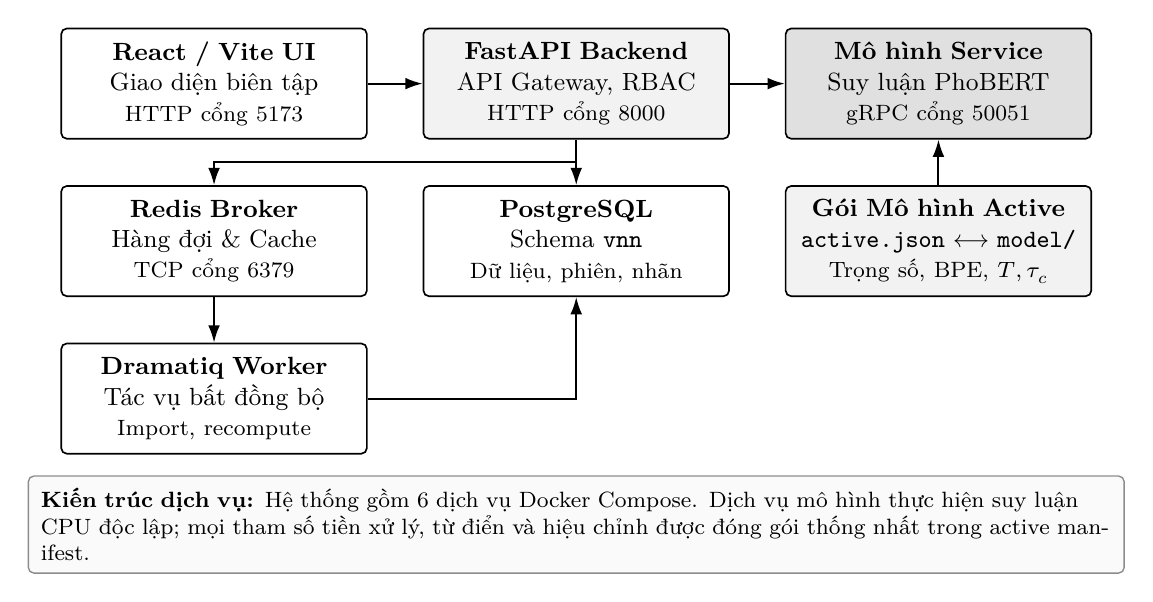
\begin{tikzpicture}
  % Column 1 (Left): Frontend & Background Queue (x = -4.6)
  \node[arch_box, text width=36mm, minimum height=14mm] (ui) at (-4.6,1.8) {
    \textbf{React / Vite UI}\\
    \small Giao diện biên tập\\
    \footnotesize HTTP cổng 5173
  };
  \node[arch_box, text width=36mm, minimum height=14mm] (redis) at (-4.6,-0.2) {
    \textbf{Redis Broker}\\
    \small Hàng đợi \& Cache\\
    \footnotesize TCP cổng 6379
  };
  \node[arch_box, text width=36mm, minimum height=14mm] (worker) at (-4.6,-2.2) {
    \textbf{Dramatiq Worker}\\
    \small Tác vụ bất đồng bộ\\
    \footnotesize Import, recompute
  };

  % Column 2 (Center): API Gateway & Database (x = 0)
  \node[arch_box_gray, text width=36mm, minimum height=14mm] (api) at (0,1.8) {
    \textbf{FastAPI Backend}\\
    \small API Gateway, RBAC\\
    \footnotesize HTTP cổng 8000
  };
  \node[arch_box, text width=36mm, minimum height=14mm] (db) at (0,-0.2) {
    \textbf{PostgreSQL}\\
    \small Schema \texttt{vnn}\\
    \footnotesize Dữ liệu, phiên, nhãn
  };

  % Column 3 (Right): Inference Service & Model Bundle (x = 4.6)
  \node[arch_box_dark, text width=36mm, minimum height=14mm] (model) at (4.6,1.8) {
    \textbf{Mô hình Service}\\
    \small Suy luận PhoBERT\\
    \footnotesize gRPC cổng 50051
  };
  \node[arch_box_gray, text width=36mm, minimum height=14mm] (artifact) at (4.6,-0.2) {
    \textbf{Gói Mô hình Active}\\
    \texttt{active.json} $\longleftrightarrow$ \texttt{model/}\\
    \footnotesize Trọng số, BPE, $T, \tau_c$
  };

  % STRICTLY ORTHOGONAL ROUTING:
  % UI -> API (10mm clean horizontal arrow)
  \draw[arch_flow] (ui) -- (api);

  % API -> Model Service (10mm clean horizontal arrow)
  \draw[arch_flow] (api) -- (model);

  % API Split Bus (y = 0.8): branch to DB and branch to Redis
  \coordinate (api_bus) at (0, 0.8);
  \draw[arch_line] (api.south) -- (api_bus);
  \draw[arch_flow] (api_bus) -- (db.north);
  \draw[arch_flow] (api_bus) -| (redis.north);

  % Redis -> Worker (Clean 6mm vertical arrow)
  \draw[arch_flow] (redis) -- (worker);

  % Worker -> DB (Strictly Orthogonal: horizontal then vertical up)
  \draw[arch_flow] (worker.east) -| (db.south);

  % Active Artifact -> Model Service (Clean 6mm vertical arrow)
  \draw[arch_flow] (artifact) -- (model);

  % Bottom Invariant Badge (y = -3.8, generous clearance from Worker)
  \node[arch_badge, text width=136mm] (badge) at (0,-3.8) {
    \textbf{Kiến trúc dịch vụ:} Hệ thống gồm 6 dịch vụ Docker Compose. Dịch vụ mô hình thực hiện suy luận CPU độc lập; mọi tham số tiền xử lý, từ điển và hiệu chỉnh được đóng gói thống nhất trong active manifest.
  };
\end{tikzpicture}
\caption{Sáu dịch vụ của ứng dụng và gói mô hình dùng cho suy luận.}
\end{figure}
}

% -----------------------------------------------------------------------------
% 13. ReviewDiagram: Editorial Loop & Provenance Tracking
% Node Sizes: Exactly 1 size (36mm x 14mm) for all 6 tracking nodes.
% Fixed Spacing: dx = 46mm (gap = 10mm), dy = 24mm (gap = 10mm).
% -----------------------------------------------------------------------------
\newcommand{\ReviewDiagram}{
\begin{figure}[tbp]\centering
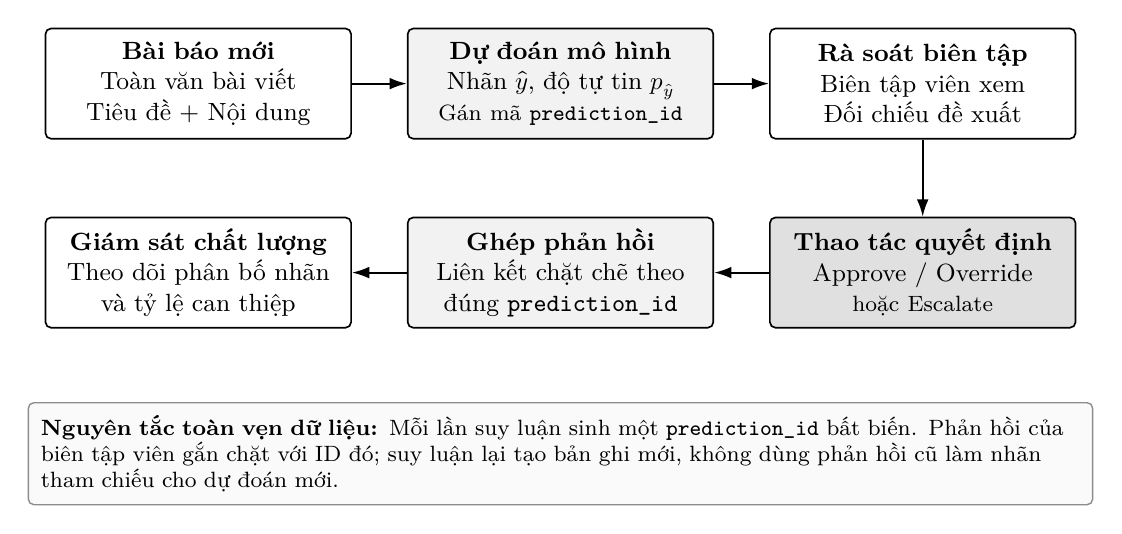
\begin{tikzpicture}
  % Upper Track: Inference & Proposal (Left to Right, y = 1.2)
  \node[arch_box, text width=36mm, minimum height=14mm] (art) at (-4.6,1.2) {
    \textbf{Bài báo mới}\\
    Toàn văn bài viết\\
    Tiêu đề + Nội dung
  };
  \node[arch_box_gray, text width=36mm, minimum height=14mm] (pred) at (0,1.2) {
    \textbf{Dự đoán mô hình}\\
    Nhãn $\hat{y}$, độ tự tin $p_{\hat{y}}$\\
    \footnotesize Gán mã \texttt{prediction\_id}
  };
  \node[arch_box, text width=36mm, minimum height=14mm] (rev) at (4.6,1.2) {
    \textbf{Rà soát biên tập}\\
    Biên tập viên xem\\
    Đối chiếu đề xuất
  };

  % Lower Track: Decision & Feedback Provenance (Right to Left, y = -1.2, exact 10mm gap!)
  \node[arch_box_dark, text width=36mm, minimum height=14mm] (dec) at (4.6,-1.2) {
    \textbf{Thao tác quyết định}\\
    Approve / Override\\
    \footnotesize hoặc Escalate
  };
  \node[arch_box_gray, text width=36mm, minimum height=14mm] (join) at (0,-1.2) {
    \textbf{Ghép phản hồi}\\
    Liên kết chặt chẽ theo\\
    đúng \texttt{prediction\_id}
  };
  \node[arch_box, text width=36mm, minimum height=14mm] (mon) at (-4.6,-1.2) {
    \textbf{Giám sát chất lượng}\\
    Theo dõi phân bố nhãn\\
    và tỷ lệ can thiệp
  };

  % Strictly Orthogonal Routing (Clean 10mm horizontal and vertical arrows)
  \draw[arch_flow] (art) -- (pred);
  \draw[arch_flow] (pred) -- (rev);
  \draw[arch_flow] (rev) -- (dec);
  \draw[arch_flow] (dec) -- (join);
  \draw[arch_flow] (join) -- (mon);

  % Invariant Badge (Spaced below join, y = -3.5, generous 9mm clearance)
  \node[arch_badge, text width=132mm] (badge) at (0,-3.5) {
    \textbf{Nguyên tắc toàn vẹn dữ liệu:} Mỗi lần suy luận sinh một \texttt{prediction\_id} bất biến. Phản hồi của biên tập viên gắn chặt với ID đó; suy luận lại tạo bản ghi mới, không dùng phản hồi cũ làm nhãn tham chiếu cho dự đoán mới.
  };
\end{tikzpicture}
\caption{Vòng phản hồi có truy vết phiên bản mô hình và lần dự đoán.}
\end{figure}
}

% -----------------------------------------------------------------------------
% 14. ActivationDiagram: Atomic Deployment & Rollback Lifecycle
% Node Sizes: Exactly 1 size (128mm x 10mm) for all 6 lifecycle stages.
% Fixed Spacing: node distance = 5.5mm.
% -----------------------------------------------------------------------------
\newcommand{\ActivationDiagram}{
\begin{figure}[tbp]\centering
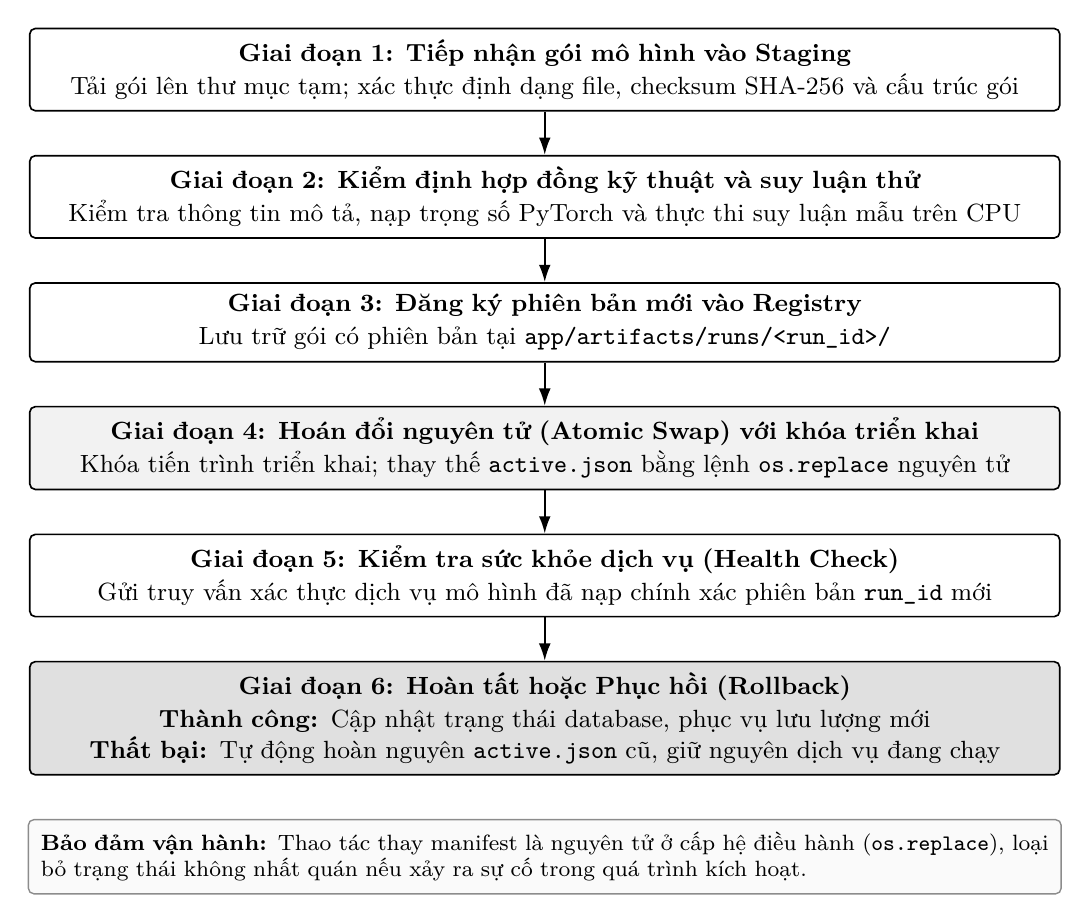
\begin{tikzpicture}[node distance=5.5mm]
  \node[arch_box, text width=128mm, minimum height=10mm] (a1) {
    \textbf{Giai đoạn 1: Tiếp nhận gói mô hình vào Staging}\\[1pt]
    Tải gói lên thư mục tạm; xác thực định dạng file, checksum SHA-256 và cấu trúc gói
  };
  \node[arch_box, text width=128mm, minimum height=10mm, below=of a1] (a2) {
    \textbf{Giai đoạn 2: Kiểm định hợp đồng kỹ thuật và suy luận thử}\\[1pt]
    Kiểm tra thông tin mô tả, nạp trọng số PyTorch và thực thi suy luận mẫu trên CPU
  };
  \node[arch_box, text width=128mm, minimum height=10mm, below=of a2] (a3) {
    \textbf{Giai đoạn 3: Đăng ký phiên bản mới vào Registry}\\[1pt]
    Lưu trữ gói có phiên bản tại \texttt{app/artifacts/runs/<run\_id>/}
  };
  \node[arch_box_gray, text width=128mm, minimum height=10mm, below=of a3] (a4) {
    \textbf{Giai đoạn 4: Hoán đổi nguyên tử (Atomic Swap) với khóa triển khai}\\[1pt]
    Khóa tiến trình triển khai; thay thế \texttt{active.json} bằng lệnh \texttt{os.replace} nguyên tử
  };
  \node[arch_box, text width=128mm, minimum height=10mm, below=of a4] (a5) {
    \textbf{Giai đoạn 5: Kiểm tra sức khỏe dịch vụ (Health Check)}\\[1pt]
    Gửi truy vấn xác thực dịch vụ mô hình đã nạp chính xác phiên bản \texttt{run\_id} mới
  };
  \node[arch_box_dark, text width=128mm, minimum height=10mm, below=of a5] (a6) {
    \textbf{Giai đoạn 6: Hoàn tất hoặc Phục hồi (Rollback)}\\[1pt]
    \textbf{Thành công:} Cập nhật trạng thái database, phục vụ lưu lượng mới\\
    \textbf{Thất bại:} Tự động hoàn nguyên \texttt{active.json} cũ, giữ nguyên dịch vụ đang chạy
  };

  % Strictly Orthogonal Straight Connections (All fixed 5.5mm vertical arrows)
  \draw[arch_flow] (a1) -- (a2);
  \draw[arch_flow] (a2) -- (a3);
  \draw[arch_flow] (a3) -- (a4);
  \draw[arch_flow] (a4) -- (a5);
  \draw[arch_flow] (a5) -- (a6);

  % Bottom Invariant Badge
  \node[arch_badge, text width=128mm, below=5.5mm of a6] (b) {
    \textbf{Bảo đảm vận hành:} Thao tác thay manifest là nguyên tử ở cấp hệ điều hành (\texttt{os.replace}), loại bỏ trạng thái không nhất quán nếu xảy ra sự cố trong quá trình kích hoạt.
  };
\end{tikzpicture}
\caption{Kiểm tra và kích hoạt một gói mô hình có kiểm soát.}
\end{figure}
}


\newcommand{\PortraitFigure}[2]{\begin{figure}[tbp]\centering
\includegraphics[width=.94\linewidth,height=.72\textheight,keepaspectratio]{#1}
\caption{#2}\end{figure}}

\newcommand{\PortraitFigureIntro}[3]{#1\PortraitFigure{#2}{#3}}
